\documentclass[licencjacka]{pracamgr}
\usepackage{polski}
\usepackage[utf8]{inputenc}
\usepackage[table]{xcolor}
\usepackage{array}
\usepackage{amssymb}
\usepackage{amsmath}
\usepackage{amsthm}
\usepackage[pdftex]{graphicx}
\usepackage{underscore}
\usepackage{hyperref}
\author{Tomasz Grabowski, Adam Markiewicz, Albert Rozmus, Krzysztof Rutkowski, Wiktor Zuba}
\nralbumu{305145, 334774, 248353, 319379, 320501}
\title{tytuł}
\tytulang{English title}
\kierunek{Informatyka}
\opiekun{dra Roberta Dąbrowskiego\\
Pion Zastępcy Kanclerza ds. Informatycznych}
\date{??? 2015}
\dziedzina{
11.0 Matematyka, Informatyka:\\
11.3 Informatyka\\
}
\klasyfikacja{
Information systems\\
Information systems applications\\
Decision support systems\\
Data analytics
}
%\TODO dodać litery/numery wierzchołków w klasyfikacji
\keywords{słowa kluczowe}
%\newtheorem{defi}{Definicja}[section]
\begin{document}
\maketitle
\begin{abstract}
Tu będzie abstract (skrót)
\end{abstract}
\tableofcontents
\chapter*{Wstęp}

Celem projektu było stworzenie serwisu internetowego 
wspierającego studentów w procesie doboru przedmiotów
i konstruowania spójnego planu zajęć.
Serwis miał za zadanie 
umożliwić studentom lepsze planowanie ścieżki studiów i kariery zawodowej
poprzez proponowanie przedmiotów, które mogą pasować do upodobań konkretnego studenta.
Propozycje zostały przydzielone na podstawie dotychczas wybieranych przedmiotów i otrzymywanych z nich ocen.
Dodatkowym wymaganiem projektu było oferowanie usług przewidywania dla konkretnych studentów ocen z przedmiotów, których jescze nie ukończyli lub nawet nie podjęli.
Ponadto serwis oferuje wsparcie dla uniwersytetu w postaci
przewidywania ilości studentów którzy zapiszą się na konkretny przedmiot.
 
\addcontentsline{toc}{chapter}{Wprowadzenie}
 \chapter{Architektura}
TODO - lepszy obrazek \newline
 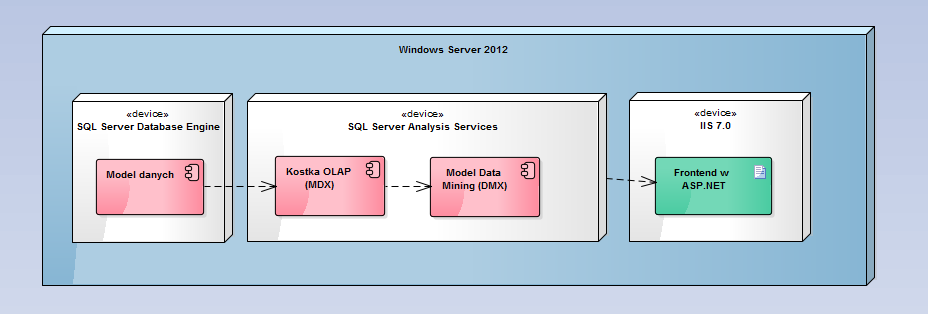
\includegraphics[scale=0.6]{Architektura.png}\newline
 W architekturze i logice naszego systemu wyróżniamy następujące komponenty:
 \begin{itemize}
 
\item \textbf{Chmura} - Sercem systemu jest główny serwer wraz z innymi usługami znajdujący się w chmurze internetowej. Znajduje się na niej serwer bazy danych, serwer WWW oraz serwer usług analitycznych.

\item \textbf {RDB} - Relacyjna baza danych zawierająca statystyczne dane dotyczące zdawalności przedmiotów przez studentów, ich zapełnienia, popularność itd. Stanowi bazę do tworzenia kostek analitycznych. 

\item \textbf {Kostka OLAP} - struktura danych, która pozwala na szybką analizę danych. Przechowuje ona dane w sposób bardziej przypominający wielowymiarowe arkusze kalkulacyjne niż tradycyjną, relacyjną bazę danych. Rozmieszczenie danych w kostkach pokonuje ograniczenia relacyjnych baz danych.

\item \textbf{Analysis Service} - usługi analityczne dokonujące analizy danych za pomocą algorytmów uczenia maszynowego oraz data mining.
 
\item \textbf{USOS Api} - API udostępniane przez system USOS. Nasz system wykorzystuje je w celu zebrania danych zalogowanego użytkownika niezbędnych do zarekomendowania mu tego czego oczekuje.

\item \textbf{Strona WWW} - interfejs za pomocą którego użytkownik może przesyłać prośby o wykonanie udostępnianych przez system rekomendacji.

\item \textbf{Serwer WWW} - udostępnia użytkownikom stronę internetową, w naszym systemie pośredniczy między interfejsem użytkownika a bazą danych.
  
\end{itemize}

Schemat działania i komunikacji między poszczególnymi komponentami wygląda następująco:
\begin{enumerate}

\item Na samym początku działania system tworzy relacyjną bazę danych zawierającą dane statystyczne z USOSa. 

\item Po stworzeniu bazy danych system wykorzystuje usługi Analysis Services w celu stworzenia kostki analitycznej.

\item Po utworzeniu kostki system wykorzystuje usługi Analisys Services w celu przeprowadzenia analizy
danych na kostce i utworzenia odpowiednich modeli predykcyjnych.

\item Po udanym stworzeniu modeli aktywuje się serwer WWW i system staje się dostępny dla użytkowników. 

\item Użytkownik wchodzi na stronę i wysyła żądanie na serwer WWW.

\item Serwer WWW generuje stronę z formularzem zalogowania się.

\item Po odebraniu danych logowania, w przypadku sukcesu, serwer pobiera dane użytkownika przez USOS Api i zwraca stronę WWW - interfejs użytkownika.

\item Serwer WWW po odebraniu prośby o rekomendacje przesyła żądanie do serwera bazy danych o dokonanie predykcji wykorzystując odebrane wcześniej dane użytkownika.

\item Serwer WWW odbiera rezultat zapytania i wyświetla go użytkownikowi.

\end{enumerate}



 \chapter{Technologia}
to tylko testowa wersja, pewnie ze wzgledu na duze przeciecie zdan z architektura bedzie potem do kosza ale kto wie \newline
Technologie wykorzystywane w naszym systemie:
\begin{itemize}

\item \textbf{Microsoft Azure} - Azure jest komercyjną platformą obsługiwaną przez Microsoft. Udostępnia ona usługi związane z chmurą internetową (tzw cloud-computing). W naszym systemie znajduje sie na niej serwer WWW a także serwer bazy danych. 

\item \textbf{Microsoft SQL Server 2014} - Komercyjny serwer bazodanowy udostępniany przez Microsoft. Znajduje się w nim relacyjna baza danych zawierająca dane niezbędne do stworzenia modelu analitycznego. 

\item \textbf{SQL Server Analysis Services} - usługi analityczne udostępniane przez SQL Server. W naszym systemie tworzą kostkę OLAP-ową usprawniającą analizę danych, którą potem wykonują.

\item \textbf {USOS Api} - API udostępniane przez system USOS. Nasz system wykorzystuje go w celu zebrania danych zalogowanego użytkownika niezbędnych do rekomendacji.

\item \textbf{ASP.NET} - technologia, za pomocą której tworzymy webowy interfejs użytkownika. W celu uzyskania możliwie dużej przenośności została zaprojektowana w metodologii RWD (Responsive Web Design).  

\end{itemize}

\begin{thebibliography}{99}
\addcontentsline{toc}{chapter}{Bibliografia}
\bibitem[MDX]{MDX} 	
\emph{Professional Microsoft SQL Server 2012 Analysis Services with MDX and DAX},
Sivakumar Harinath, Ronald Pihlgren, Denny Guang-Yeu Lee, John Sirmon, Robert M. Bruckner,
October 2012
\bibitem[SSAS]{SSAS} 
\emph{Expert Cube Development with SSAS Multidimensional Models},
Chris Webb, Alberto Ferrari, Marco Russo,
February 2014
\bibitem[SQL2014]{SQL2014} 
\emph{Professional Microsoft SQL Server 2014 Integration Services},
Brian Knight, Devin Knight, Jessica M. Moss, Mike Davis, Chris Rock,
June 2014
\bibitem[technet]{technet}
http://technet.microsoft.com/en-us/sqlserver/cc510300.aspx
\bibitem[ASP.NET]{ASP.NET}
http://www.asp.net/mvc
\end{thebibliography}
\end{document}